

\section{Introduction} \label{Intro}
	We are interested here in finding an algorithm to decide if a phase transition occurred in a material between two different temperatures. The data structure is given by different curves of Intensity (I) as a function of distance (d - characteristic spacing of the material in Angstroms) for different values of temperature (T).
To define a phase transition we first study one particular peak in the intensity curves, namely the peak between 3.2 and 3.3 ${\AA}$. The characterization of this peak consists of calculating its center, a characteristic width and the area under it.
Once we have the characterization procedure we move on  characterize all the peaks in the data set for a given temperature value. Finally, one can define a phase transition by looking at the sets of peaks and its characteristics for two different adjacent curves (temperatures). We define a phase transition as a distinct change in structure of the intensity peaks.

\section{Inspecting the Data} \label{Data}
	Before we inspect any particular peaks, let us look at different sets of curves for randomly chosen values of temperatures to understand how the peak structure is. Figure \ref{fig:randTs}  shows the curves of intensity as a function of d-spacing for random values of T.

\begin{figure}[h]
  \centering
  %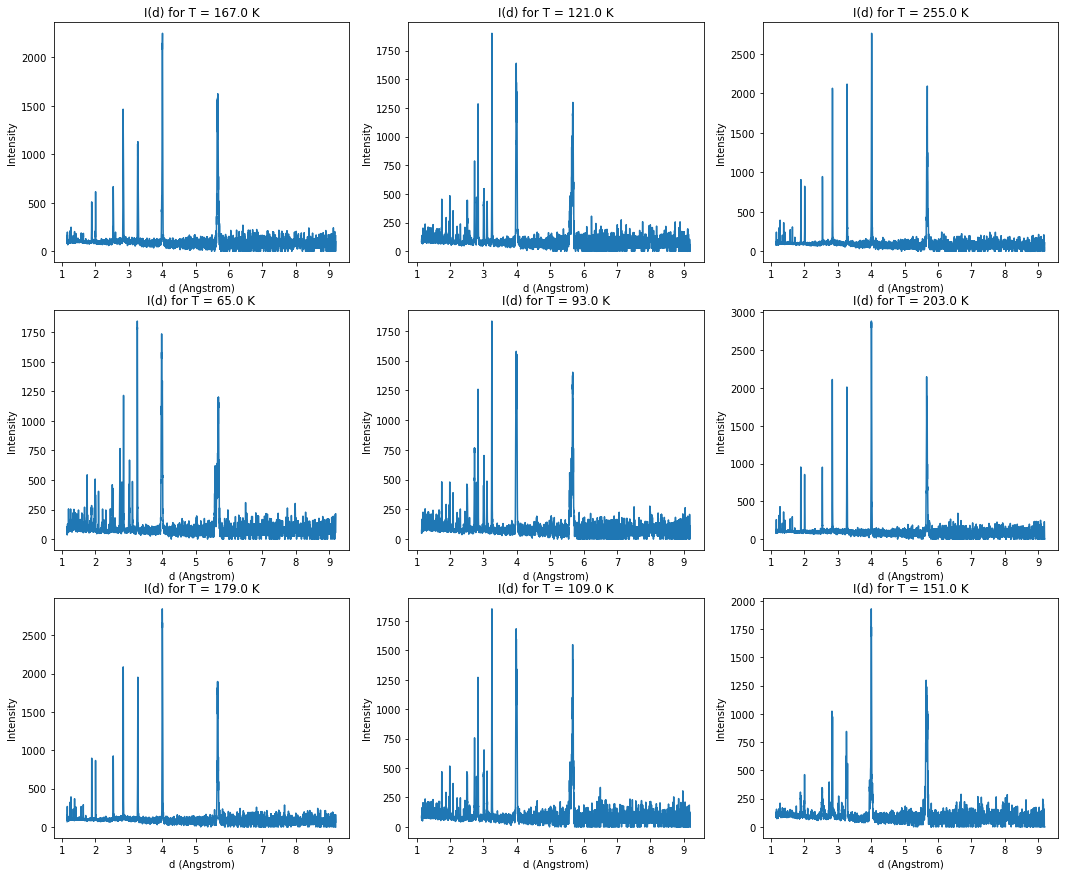
\includegraphics[scale=0.25, width=0.8\linewidth]{../figs/randomTs.png}
  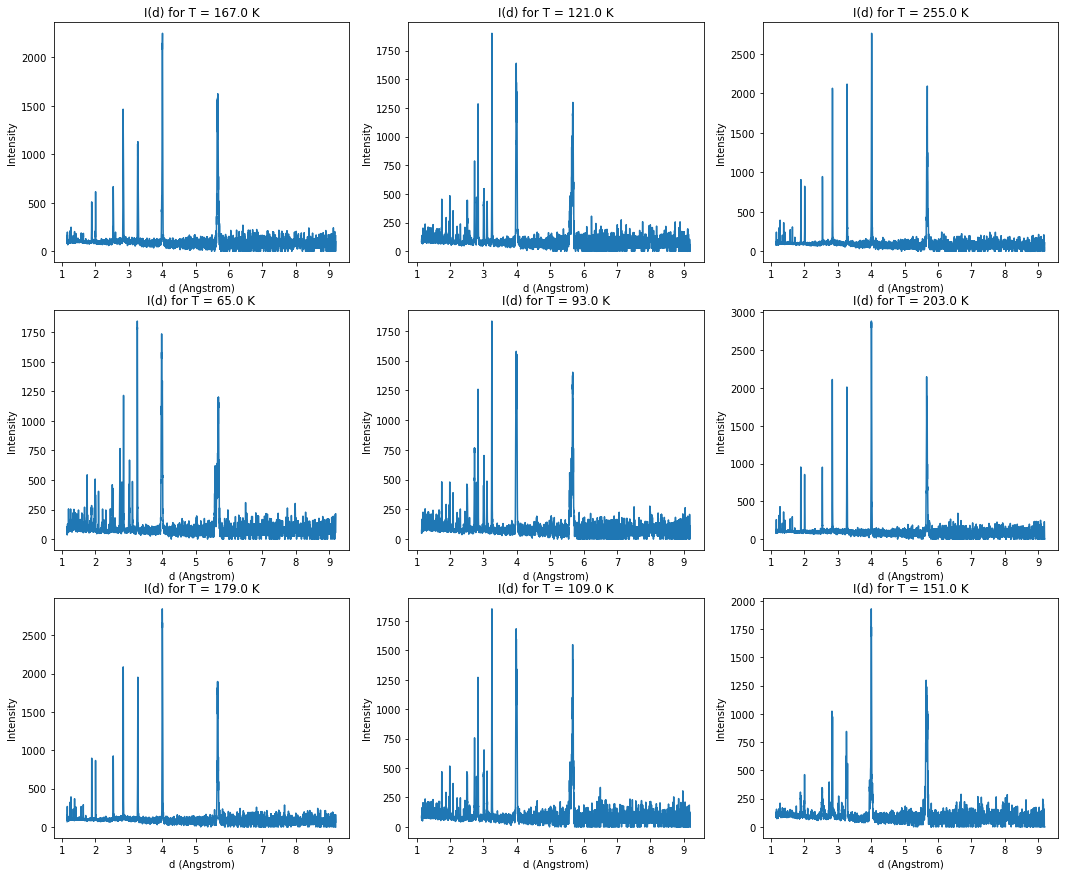
\includegraphics[scale=0.25]{../figs/randomTs.png}
  \caption{Intensity curves as a function of d-spacing for different values of temperature.}
  \label{fig:randTs}
\end{figure}

We can also look at the maximum intensity distribution as a function of temperature. Figure \ref{fig:maxI} shows the highest value of I for each temperature T. We can already see a big hint of a structure change at around $\textrm{T} = 150 \textrm{ K}$. This particular data set has a unique maximum intensity value for each temperature. This allows us to uniquely map a temperature to an intensity value and vice-versa. So given a temperature value we can find the corresponding set of intensity values or the opposite.
This is certainly not a general result valid for any data set, but it is valid for the particular one that we are working with here. Building this one-to-one map makes it faster to get a curve given a temperature and also scales a lot faster with more data, in case the new data also presents this feature.

\begin{figure}[h]
  \centering
  %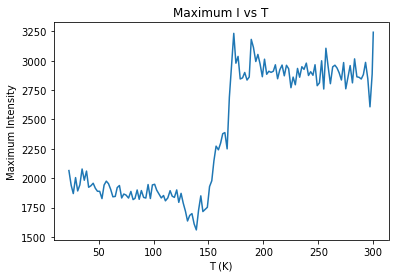
\includegraphics[scale=0.1, width=0.8\linewidth]{../figs/maxI.png}
  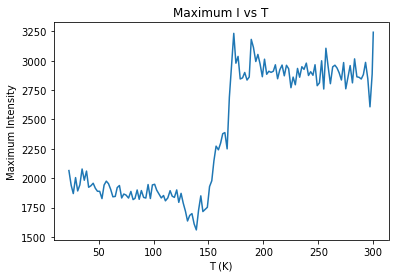
\includegraphics[scale=0.25]{../figs/maxI.png}
  \caption{Maximum intensity value as a function of function temperature.}
  \label{fig:maxI}
\end{figure}